\documentclass[11pt]{article}

\usepackage[a4paper,margin=1in]{geometry}
\usepackage{amsmath,amssymb,amsthm,mathtools}
\usepackage{microtype}
\usepackage{booktabs}
\usepackage{enumitem}
\usepackage{xcolor}
\usepackage{tikz}
\usepackage{hyperref}
\usepackage{cleveref}
\usepackage{array}

\hypersetup{
  colorlinks=true,
  linkcolor=blue!55!black,
  citecolor=blue!55!black,
  urlcolor=blue!55!black,
  pdftitle={An Elementary ln(2) Volumetric-History Adversary for Comparison Sorting},
  pdfauthor={Nicholas Nash and OpenAI GPT-5.6 Pro}
}

\definecolor{deepblue}{RGB}{30,70,120}
\definecolor{softblue}{RGB}{235,243,252}
\definecolor{softgray}{RGB}{246,246,246}

\newtheorem{theorem}{Theorem}[section]
\newtheorem{lemma}[theorem]{Lemma}
\newtheorem{proposition}[theorem]{Proposition}
\newtheorem{corollary}[theorem]{Corollary}
\theoremstyle{definition}
\newtheorem{definition}[theorem]{Definition}
\newtheorem{remark}[theorem]{Remark}

\newcommand{\R}{\mathbb{R}}
\newcommand{\E}{\mathbb{E}}
\newcommand{\Var}{\operatorname{Var}}
\newcommand{\tr}{\operatorname{tr}}
\newcommand{\im}{\operatorname{im}}
\newcommand{\1}{\mathbf{1}}
\newcommand{\dd}{\,\mathrm{d}}
\newcommand{\norm}[1]{\left\lVert #1\right\rVert}
\newcommand{\ip}[2]{\left\langle #1,#2\right\rangle}
\newcommand{\rhoFn}{\rho}

\title{\textbf{An Elementary $\boldsymbol{\ln 2}$ Volumetric-History Adversary\\for Comparison Sorting}\\[0.45em]
\large A second simplification of the curvature argument}
\author{Nicholas Nash\\with mathematical development and audit assistance from OpenAI GPT-5.6 Pro}
\date{August 2026}

\begin{document}
\maketitle

\begin{abstract}
We give a deterministic polynomial-time adversary for comparison sorting that forces
\[
 (\ln 2)n\log_2 n-O(n)
 =0.693147180559945\ldots\,n\log_2 n-O(n)
\]
comparisons.  The starting point is the curvature-enhanced volumetric-history method, whose stronger checkpoint coefficient is $0.6944681307\ldots$ and whose final scalar step was originally certified by 60,000 directed-rounding intervals.  We accept the very small loss from $0.694468\ldots$ to $\ln 2$ and simplify the proof further.

The potential is presented as the logarithm of a weighted spanning-tree count.  The high-dimensional comparison analysis reduces to one elementary projection identity.  Near the separating hyperplane, the two trial branches are averaged so that their cubic terms cancel; the special $4/5$ schedule makes every remaining power-series coefficient nonnegative.  The resulting scalar estimate is proved by two short logarithmic majorizations and a degree-six polynomial whose shape is immediate from the sign of its third derivative.  Away from the hyperplane, a single fixed target slack $3/4$ gives a much easier one-sided argument.  No interval arithmetic, exhaustive case analysis, long Taylor certificate, or high-degree polynomial positivity check remains.
\end{abstract}

\vspace{0.5em}
\noindent
\fcolorbox{deepblue}{softblue}{\parbox{0.94\textwidth}{
\textbf{Status.}  The mathematical proof below is fully analytic.  The transcription-sensitive identities have been checked symbolically, and the scalar inequalities and projection identity have been tested independently by the accompanying script.  The script is an audit aid, not part of the proof.  As in the stronger source checkpoint, the polynomial-time implementation uses standard deterministic convex minimization to approximate the current center.  A publication version should still receive an independent line-by-line audit, especially of the approximation/bit-complexity paragraph.
}}

\tableofcontents

\section{What changed in this simplification}

The stronger curvature checkpoint proves a coefficient
\[
0.694468130795582\ldots
\]
by showing that every informative comparison increases the base-$2$ potential by at most
\[
\frac12\log_2(7.361)=1.4399508856\ldots .
\]
Its higher-dimensional argument is exact; only the final one-variable estimate uses a computer-assisted interval certificate \cite{NashCurvature2026}.  The present memo targets the slightly larger determinant budget
\[
e^2=7.3890560989\ldots,
\]
which corresponds exactly to a unit increase in the natural-log potential and hence to leading coefficient $\ln 2$ in base $2$.

The new proof has four reductions.

\begin{enumerate}[label=\textbf{\arabic*.},leftmargin=2.3em]
\item The volumetric determinant is the weighted spanning-tree partition function of a graph built from the comparison history.
\item Whitening one query leaves only numbers $\alpha_i\in[-1,1]$ satisfying $\sum_i\alpha_i^2=1$.
\item A one-line weighted average cancels the only uncontrolled moment, $\sum_i\alpha_i^3$.
\item The offset range is split at $\delta=1/4$ and $\delta=3/4$.  Only $0\le\delta\le1/4$ needs the two-branch calculation; the rest is handled by a fixed one-sided move or no move at all.
\end{enumerate}

The last reduction is the decisive new simplification.  It shrinks the delicate scalar interval enough that a transparent degree-six majorant has ample slack.

\section{The history as a weighted graph}

Let $V=[n]$ be the items.  The adversary retains every informative comparison it has answered.  If it answered $u<v$, the directed edge $u\to v$ remains in the history even after becoming transitively redundant.  The retained edges form a directed acyclic graph $G$.

Introduce a coordinate $x_v\in(0,1)$ for every item.  The open history region is
\[
K_G=\{x\in(0,1)^n:x_u<x_v\text{ for every retained }u\to v\}.
\]

Add one ground vertex $g$.  At a feasible placement $x\in K_G$, construct a multigraph $\Gamma_G(x)$ as follows.

\begin{itemize}[leftmargin=2em]
\item For every item $v$, add two parallel edges $gv$, of lengths $x_v$ and $1-x_v$.
\item For every retained comparison $u<v$, add the edge $uv$, of length $x_v-x_u$.
\end{itemize}

An edge $e$ of length $s_e$ receives conductance $w_e=s_e^{-2}$.  Define the \emph{tree score}
\begin{equation}
Z_G(x)=\sum_{T\text{ spanning tree of }\Gamma_G(x)}\prod_{e\in T}s_e(x)^{-2}.
\label{eq:tree-score}
\end{equation}

Let $H_G(x)$ be the reduced weighted Laplacian, with the ground row and column deleted.  The weighted matrix-tree theorem gives
\begin{equation}
Z_G(x)=\det H_G(x).
\label{eq:matrix-tree}
\end{equation}
Equivalently, if every old inequality is written $a_i^Tx>b_i$ with slack $s_i(x)=a_i^Tx-b_i$, then
\begin{equation}
H_G(x)=\sum_i\frac{a_i a_i^T}{s_i(x)^2}.
\label{eq:hessian}
\end{equation}

\begin{definition}[Tree center and potential]
A \emph{tree center} of $G$ is any minimizer $x^\star\in K_G$ of $Z_G(x)$.  Define
\begin{equation}
\Psi(G)=\min_{x\in K_G}\frac12\ln Z_G(x)
       =\min_{x\in K_G}\frac12\ln\det H_G(x).
\label{eq:potential}
\end{equation}
\end{definition}

This is exactly the natural-log volumetric potential, but the tree formulation makes its discrete content visible.

\subsection{Convexity without volumetric-barrier machinery}

For a fixed spanning tree $T$, put
\[
\phi_T(x)=-2\sum_{e\in T}\ln s_e(x).
\]
Then $Z_G(x)=\sum_T e^{\phi_T(x)}$.  Along any line $x(t)$ contained in $K_G$, let a random tree $\mathcal T$ have probability proportional to $e^{\phi_T(x(t))}$.  Direct differentiation gives
\begin{equation}
\frac{\dd^2}{\dd t^2}\ln Z_G(x(t))
 =\E\bigl[\phi_{\mathcal T}''(t)\bigr]
  +\Var\bigl(\phi_{\mathcal T}'(t)\bigr)
 \ge0.
\label{eq:tree-convexity}
\end{equation}
Indeed, every slack is positive affine along the line, so $-\ln s_e$ is convex.  Thus $\ln Z_G$ is convex by a finite probabilistic calculation.

The score tends to infinity at the boundary of $K_G$.  Every retained edge belongs to some spanning tree because the box edges connect every vertex to the ground; if its slack tends to zero, at least one tree term diverges.  Hence a tree center exists in the interior.

\section{The endpoint gap}

\subsection{Initial score}

Initially there are no comparison edges.  A spanning tree chooses independently one of the two ground edges incident with each item.  Therefore
\[
Z_{G_0}(x)=\prod_{v=1}^n\left(\frac1{x_v^2}+\frac1{(1-x_v)^2}\right).
\]
Each factor is minimized at $x_v=1/2$, where it equals $8$.  Hence
\begin{equation}
\Psi(G_0)=\frac12\ln 8^n=\frac32n\ln2.
\label{eq:initial}
\end{equation}

\subsection{Terminal score}

Suppose the transcript has determined
\[
v_1<v_2<\cdots<v_n.
\]
Every adjacent relation $v_j<v_{j+1}$ must have been compared directly.  Otherwise a directed path of length at least two would contain an item strictly between two adjacent elements of the final order.

Keep only the following $n+1$ history edges:
\[
gv_1,\quad v_1v_2,\quad\ldots,\quad v_{n-1}v_n,\quad v_ng.
\]
They form a cycle.  Write their positive lengths as
\[
s_0=x_{v_1},\qquad
s_j=x_{v_{j+1}}-x_{v_j}\ (1\le j<n),\qquad
s_n=1-x_{v_n}.
\]
Then $\sum_{j=0}^n s_j=1$.  A spanning tree of the cycle is obtained by deleting one edge, so its tree score is
\begin{equation}
Z_{\mathrm{cyc}}
 =\left(\prod_{j=0}^n s_j^{-2}\right)
  \left(\sum_{j=0}^n s_j^2\right).
\label{eq:cycle-score}
\end{equation}
AM--GM and Cauchy--Schwarz give
\[
\prod_{j=0}^n s_j\le(n+1)^{-(n+1)},
\qquad
\sum_{j=0}^n s_j^2\ge\frac1{n+1}.
\]
Every tree counted in \eqref{eq:cycle-score} is also present in the full history graph.  Thus
\begin{equation}
\Psi(G_T)\ge\left(n+\frac12\right)\ln(n+1).
\label{eq:terminal}
\end{equation}
Combining \eqref{eq:initial} and \eqref{eq:terminal}, sorting requires a potential increase
\begin{equation}
\Psi(G_T)-\Psi(G_0)=n\ln n-O(n).
\label{eq:endpoint-gap}
\end{equation}

\section{Normalize one comparison}

Fix a current tree center $x^\star$ and write
\[
H=H_G(x^\star).
\]
Suppose the sorting algorithm compares two currently incomparable items.  Let $q$ be their difference vector, oriented so that
\[
q^Tx^\star\ge0.
\]
Define
\begin{equation}
R=q^TH^{-1}q,
\qquad
d=\frac{H^{-1}q}{\sqrt R},
\qquad
\delta=\frac{q^Tx^\star}{\sqrt R}\ge0.
\label{eq:electrical}
\end{equation}
Here $R$ is the effective resistance of the query and $d$ is its unit-energy electrical displacement.

For every old row $i$, set
\begin{equation}
u_i=\frac{H^{-1/2}a_i}{s_i(x^\star)},
\qquad
c=\frac{H^{-1/2}q}{\sqrt R},
\qquad
\alpha_i=u_i^Tc,
\qquad
\sigma_i=\norm{u_i}^2.
\label{eq:whitening}
\end{equation}
Then
\begin{equation}
\sum_i u_i u_i^T=I,
\qquad
\norm{c}=1,
\qquad
\sum_i\alpha_i^2=1.
\label{eq:isotropy}
\end{equation}
In particular, $|\alpha_i|\le1$.

The center condition is equally simple.  Moving along $d$ changes old slack $i$ by the factor $1+s\alpha_i$.  Differentiating $\frac12\ln\det H_G(x^\star+sd)$ at $s=0$ gives
\begin{equation}
\sum_i\sigma_i\alpha_i=0.
\label{eq:center-balance}
\end{equation}
Thus a tree center is balanced in every electrical direction.

Along the line $x(s)=x^\star+sd$,
\begin{equation}
s_i(x(s))=s_i(x^\star)(1+s\alpha_i),
\qquad
q^Tx(s)=\sqrt R(\delta+s).
\label{eq:slack-motion}
\end{equation}
Every $|s|<1$ preserves all old inequalities.

Suppose a trial point in one child gives the new query edge normalized length $t>0$.  Relative to the old Hessian, the augmented matrix is
\begin{equation}
M_t(s)=\frac{cc^T}{t^2}
       +\sum_i\frac{u_i u_i^T}{(1+s\alpha_i)^2},
\qquad
F_t(s)=\ln\det M_t(s).
\label{eq:Mt}
\end{equation}
The quantity $F_t(s)$ is exactly the natural logarithm of the determinant ratio between that trial child and the current state.

\begin{figure}[t]
\centering
\begin{tikzpicture}[x=1.15cm,y=1cm,>=stealth]
  \draw[->,thick] (-4.2,0) -- (5.3,0) node[right] {$q^Tx/\sqrt R$};
  \draw[thick] (0,-0.15)--(0,0.15) node[below=5pt] {$0$};
  \draw[thick] (1.3,-0.15)--(1.3,0.15) node[below=5pt] {$\delta$};
  \draw[thick,deepblue] (3.7,-0.15)--(3.7,0.15) node[below=5pt] {$t_+$};
  \draw[thick,deepblue] (-2.7,-0.15)--(-2.7,0.15) node[below=5pt] {$-t_-$};
  \draw[<->,deepblue] (1.3,0.55)--(3.7,0.55) node[midway,above] {$a=t_+-\delta$};
  \draw[<->,deepblue] (-2.7,0.95)--(1.3,0.95) node[midway,above] {$b=t_-+\delta$};
  \node[align=center] at (0.45,-1.15) {old center};
\end{tikzpicture}
\caption{The normalized query line.  The center lies at $\delta\ge0$.  The positive trial moves by $a$ and finishes at slack $t_+$; the negative trial moves by $-b$ and finishes at slack $t_-$.}
\label{fig:query-line}
\end{figure}

\section{The one high-dimensional lemma}

The following is the only part of the proof that is not scalar calculus or elementary graph theory.

\begin{lemma}[Projection curvature]
For every admissible $s$,
\begin{equation}
F_t''(s)\le3\sum_i\frac{\alpha_i^2}{(1+s\alpha_i)^2}.
\label{eq:curvature-bound}
\end{equation}
\end{lemma}

\begin{proof}
Let $B_s$ be the matrix whose rows are
\[
\frac{c^T}{t},
\qquad
\frac{u_i^T}{1+s\alpha_i}.
\]
Then $M_t(s)=B_s^TB_s$.  Put
\[
P_s=B_s(B_s^TB_s)^{-1}B_s^T,
\qquad
D_s=\operatorname{diag}\left(0,
\frac{\alpha_1}{1+s\alpha_1},\ldots,
\frac{\alpha_m}{1+s\alpha_m}\right).
\]
The matrix $P_s$ is the orthogonal projection onto the column space of $B_s$.  Differentiating the row scales gives
\[
M_t'(s)=-2B_s^TD_sB_s,
\qquad
M_t''(s)=6B_s^TD_s^2B_s.
\]
Therefore
\begin{equation}
F_t''(s)=6\tr(P_sD_s^2)-4\tr(P_sD_sP_sD_s).
\label{eq:exact-curvature}
\end{equation}
Choose coordinates in edge space in which $P_s=\operatorname{diag}(I,0)$ and write
\[
D_s=\begin{pmatrix}A&B\\B^T&C\end{pmatrix}.
\]
Then \eqref{eq:exact-curvature} becomes
\[
F_t''(s)=2\norm{A}_F^2+6\norm{B}_F^2.
\]
Since
\[
\norm{D_s}_F^2=\norm{A}_F^2+2\norm{B}_F^2+\norm{C}_F^2,
\]
we obtain
\[
F_t''(s)\le3\norm{D_s}_F^2
=3\sum_i\frac{\alpha_i^2}{(1+s\alpha_i)^2}.
\]
\end{proof}

\begin{remark}
The proof is just Pythagoras for an orthogonal projection.  The factor $3$ is the only genuine quantitative loss in the high-dimensional part.  Everything that follows is one-dimensional.
\end{remark}

\section{Integrating the curvature}

At $s=0$,
\[
M_t(0)=I+\frac{cc^T}{t^2},
\qquad
F_t(0)=\ln(1+t^{-2}).
\]
The Sherman--Morrison formula gives
\[
M_t(0)^{-1}=I-\frac{cc^T}{1+t^2}.
\]
Using the balance identity \eqref{eq:center-balance},
\begin{align}
F_t'(0)
&=-2\sum_i\alpha_i\left(\sigma_i-\frac{\alpha_i^2}{1+t^2}\right)\\
&=\frac{2}{1+t^2}\sum_i\alpha_i^3.
\label{eq:first-derivative}
\end{align}
Write
\[
m_3=\sum_i\alpha_i^3,
\qquad
\rho(z)=z-\ln(1+z).
\]
Integrating \eqref{eq:curvature-bound} twice yields the following.

\begin{proposition}[Two branch bounds]
For $0\le a,b<1$,
\begin{align}
F_t(a)
&\le \ln(1+t^{-2})
 +\frac{2a}{1+t^2}m_3
 +3\sum_i\rho(a\alpha_i),
\label{eq:positive-integrated}\\
F_t(-b)
&\le \ln(1+t^{-2})
 -\frac{2b}{1+t^2}m_3
 +3\sum_i\rho(-b\alpha_i).
\label{eq:negative-integrated}
\end{align}
\end{proposition}

\begin{proof}
The only calculation is
\[
\int_0^a(a-s)\frac{\alpha^2}{(1+s\alpha)^2}\dd s
=a\alpha-\ln(1+a\alpha)=\rho(a\alpha),
\]
and the analogous identity on $[-b,0]$.
\end{proof}

\section{Cubic cancellation as a positive-series lemma}

The next lemma compresses both the cancellation of $m_3$ and the elimination of all frame dependence.

\begin{lemma}[Two-trial positive-series lemma]
Let $t_+,t_->0$ and
\[
a=t_+-\delta,
\qquad
b=t_-+\delta,
\qquad
0<a\le b<1.
\]
Put
\[
A=\frac{a}{1+t_+^2},
\qquad
B=\frac{b}{1+t_-^2},
\qquad
\lambda=\frac{B}{A+B}.
\]
Assume
\begin{equation}
b^2(1+t_-^2)\ge a^2(1+t_+^2).
\label{eq:cubic-condition}
\end{equation}
Then
\begin{align}
\min\{F_{t_+}(a),F_{t_-}(-b)\}
\le{}&\lambda\bigl[\ln(1+t_+^{-2})+3\rho(a)\bigr]\\
&+(1-\lambda)\bigl[\ln(1+t_-^{-2})+3\rho(-b)\bigr].
\label{eq:two-trial-scalar}
\end{align}
\end{lemma}

\begin{proof}
Take the weighted average of \eqref{eq:positive-integrated} and \eqref{eq:negative-integrated}.  Since
\[
\lambda\frac{a}{1+t_+^2}
=(1-\lambda)\frac{b}{1+t_-^2},
\]
the $m_3$ terms cancel.

It remains to bound
\[
h(z)=\lambda\rho(az)+(1-\lambda)\rho(-bz).
\]
The power series $\rho(w)=\sum_{k\ge2}(-1)^kw^k/k$ gives
\[
h(z)=\sum_{k\ge2}\frac{c_kz^k}{k},
\qquad
c_k=\lambda(-1)^ka^k+(1-\lambda)b^k.
\]
Even coefficients are positive.  For odd $k\ge3$, condition \eqref{eq:cubic-condition} is exactly $c_3\ge0$; because $b\ge a$, it then implies $c_k\ge0$ for every larger odd $k$.

Thus all $c_k$ are nonnegative.  For $0\le z\le1$, $z^k\le z^2$, so $h(z)\le z^2h(1)$.  For $-1\le z<0$, the odd terms only decrease $h(z)$, while the even terms are at most $z^2$ times their value at $1$.  Hence again $h(z)\le z^2h(1)$.  Finally,
\[
\sum_i h(\alpha_i)\le h(1)\sum_i\alpha_i^2=h(1),
\]
which proves \eqref{eq:two-trial-scalar}.
\end{proof}

The cancellation is therefore not mysterious: choose the averaging weights so that the cubic terms balance, and choose the trial geometry so that every higher coefficient has the correct sign.

\section{The explicit adversary rule}

For an informative query, orient $q$ so that $\delta\ge0$ and use the following rule.

\begin{center}
\begin{tabular}{>{\raggedright\arraybackslash}p{0.19\textwidth} >{\raggedright\arraybackslash}p{0.69\textwidth}}
\toprule
Offset & Response rule \\
\midrule
$0\le\delta\le1/4$
& Let $r=1/\sqrt3$.  Form the positive trial
$x_+=x^\star+(r-\delta/5)d$
and the negative trial
$x_-=x^\star-(r+\delta/5)d$.
Compute the two trial determinants and choose the smaller.\\[0.4em]
$1/4\le\delta\le3/4$
& Answer in the positive direction and move to
$x^\star+(3/4-\delta)d$, so that the final normalized query slack is exactly $3/4$.\\[0.4em]
$\delta\ge3/4$
& Answer in the positive direction and do not move the center.\\
\bottomrule
\end{tabular}
\end{center}

The overlaps at $1/4$ and $3/4$ are harmless; either adjacent rule works.

\begin{figure}[t]
\centering
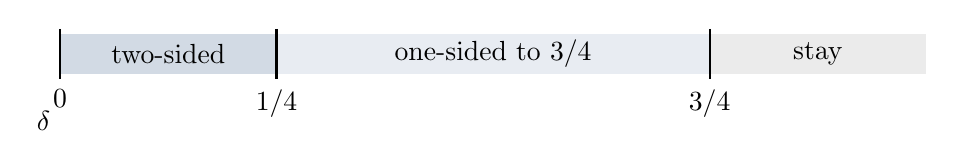
\begin{tikzpicture}[x=11cm,y=1cm]
  \draw[thick] (0,0)--(0.25,0)--(0.75,0)--(1,0);
  \fill[deepblue!20] (0,-0.25) rectangle (0.25,0.25);
  \fill[deepblue!10] (0.25,-0.25) rectangle (0.75,0.25);
  \fill[black!8] (0.75,-0.25) rectangle (1,-0.25+0.5);
  \draw[thick] (0,0.32)--(0,-0.32) node[below] {$0$};
  \draw[thick] (0.25,0.32)--(0.25,-0.32) node[below] {$1/4$};
  \draw[thick] (0.75,0.32)--(0.75,-0.32) node[below] {$3/4$};
  \node at (0.125,0) {two-sided};
  \node at (0.50,0) {one-sided to $3/4$};
  \node at (0.875,0) {stay};
  \node[left] at (0,-0.85) {$\delta$};
\end{tikzpicture}
\caption{The simplified offset strategy.  The delicate two-branch estimate is needed only on $[0,1/4]$.}
\label{fig:regimes}
\end{figure}

\section{The central regime: a six-term majorant}

Assume $0\le\delta\le1/4$ and put
\begin{equation}
r=\frac1{\sqrt3},
\qquad
y=\frac{\sqrt3\,\delta}{5}.
\label{eq:y-def}
\end{equation}
Then $0\le y\le Y:=\sqrt3/20$ and the two trials are
\begin{equation}
 t_+=r(1+4y),\qquad t_-=r(1-4y),
\qquad a=r(1-y),\qquad b=r(1+y).
\label{eq:four-fifths}
\end{equation}
They are feasible: $t_->0$, $a>0$, and $b<1$.

The special role of the $4/5$ schedule is the exact identity
\begin{equation}
b^2(1+t_-^2)-a^2(1+t_+^2)=\frac{16}{3}y^3\ge0.
\label{eq:magic-cubic}
\end{equation}
Thus the positive-series lemma applies.

Define
\[
U(t)=\ln(1+t^{-2}),
\qquad
X(y)=U(t_+)+3\rho(a),
\qquad
Y(y)=U(t_-)+3\rho(-b).
\]
A direct simplification gives
\begin{equation}
2\lambda-1=\eta(y):=\frac{y(3+4y^2)}{1+6y^2}.
\label{eq:eta}
\end{equation}
Writing
\[
S=\frac{X+Y}{2},
\qquad
D=\frac{X-Y}{2},
\qquad
L=S+\eta D,
\]
Lemma 7.1 gives
\begin{equation}
\min\{F_{t_+}(a),F_{t_-}(-b)\}\le L(y).
\label{eq:min-L}
\end{equation}

Put
\[
L_0=\ln4+\frac32\ln\frac32,
\qquad
D_0=\sqrt3-\frac32\ln(2+\sqrt3),
\]
\[
\beta=\frac{\sqrt3+1}{2},
\qquad
\gamma=\frac{\sqrt3-1}{2}.
\]
Elementary multiplication of the logarithms gives
\begin{align}
S(y)=L_0
&+\frac12\ln(1+4y^2+16y^4)-\ln(1-16y^2)\notag\\
&-\sqrt3\,y-\frac32\ln\left(1-\sqrt3\,y+\frac12y^2\right),
\label{eq:S-formula}\\[0.4em]
D(y)=D_0
&+\frac12\ln\frac{1+2y+4y^2}{1-2y+4y^2}
 -\ln\frac{1+4y}{1-4y}\notag\\
&+\frac32\ln\frac{1-\beta y}{1-\gamma y}.
\label{eq:D-formula}
\end{align}

The next lemma is the entire scalar certificate.

\begin{lemma}[Six-term central majorant]
For $0\le y\le\sqrt3/20$,
\begin{equation}
L(y)\le L_0+P(y),
\label{eq:majorant}
\end{equation}
where
\begin{equation}
P(y)=\frac7{50}y-3y^2+y^3+111y^4+21y^5+2167y^6.
\label{eq:P}
\end{equation}
Moreover,
\begin{equation}
P(y)<\frac1{500}
\qquad\text{and}\qquad
L_0<\frac{399}{200}.
\label{eq:P-L0-bounds}
\end{equation}
Consequently $L(y)<1.997<2$ throughout the central regime.
\end{lemma}

\begin{proof}
Let $N(z)=-\ln(1-z)=\sum_{k\ge1}z^k/k$.  We repeatedly use
\begin{equation}
N(z)\le\sum_{k=1}^{m-1}\frac{z^k}{k}
      +\frac{z^m}{m(1-z)},
\qquad 0\le z<1,
\label{eq:N-tail}
\end{equation}
and $\ln(1+z)\le z$.

Because $16y^2\le3/25$ and $\beta y\le(3+\sqrt3)/40<1/8$, equation \eqref{eq:S-formula} gives
\begin{align}
S(y)\le L_0
&+\frac{\sqrt3}{2}y+\frac{39}{2}y^2
 +\frac{3\sqrt3}{4}y^3+\frac{2197}{16}y^4\notag\\
&+2y^5+1552y^6.
\label{eq:S-upper}
\end{align}
Here are the two tail estimates behind \eqref{eq:S-upper}.  First,
\[
N(16y^2)
\le16y^2+128y^4
 +\frac{4096y^6}{3(1-3/25)}
<16y^2+128y^4+1552y^6.
\]
Second,
\[
\frac32\sum_{k\ge5}\frac{(\beta^k+\gamma^k)y^k}{k}
\le\frac{12}{35}(\beta^5+\gamma^5)y^5
=\frac{33\sqrt3}{35}y^5<2y^5.
\]
We used $\beta^5+\gamma^5=11\sqrt3/4$.

For $D$, define
\[
A(y)=\frac12\ln\frac{1+2y+4y^2}{1-2y+4y^2}.
\]
Then
\[
A'(y)=\frac{2(1-4y^2)}{1+4y^2+16y^4}\le2,
\]
so $A(y)\le2y$.  Expanding only terms that occur with a negative sign in \eqref{eq:D-formula},
\[
-\ln\frac{1+4y}{1-4y}
\le-8y-\frac{128}{3}y^3,
\]
and
\[
\frac32\ln\frac{1-\beta y}{1-\gamma y}
\le-\frac32y-\frac{3\sqrt3}{4}y^2-\frac54y^3.
\]
Therefore
\begin{equation}
D(y)\le D_*(y):=
D_0-\frac{15}{2}y-\frac{3\sqrt3}{4}y^2-\frac{527}{12}y^3<0.
\label{eq:D-upper}
\end{equation}
The last sign follows from
\[
\frac12\ln(2+\sqrt3)
=\operatorname{artanh}\frac1{\sqrt3}
>\frac1{\sqrt3},
\]
which implies $D_0<0$.

From \eqref{eq:eta},
\begin{equation}
\eta(y)=3y-\frac{14y^3}{1+6y^2}
\ge3y-14y^3=:p(y)>0.
\label{eq:eta-lower}
\end{equation}
Since both $D$ and $D_*$ are negative,
\[
\eta D\le pD\le pD_*.
\]
Combining this with \eqref{eq:S-upper} and collecting powers gives
\begin{align}
L(y)\le L_0
&+c_1y-3y^2+c_3y^3+\frac{1769}{16}y^4\notag\\
&+\left(2+\frac{21\sqrt3}{2}\right)y^5
 +\frac{13001}{6}y^6,
\label{eq:pre-P}
\end{align}
where
\[
c_1=\frac{7\sqrt3}{2}-\frac92\ln(2+\sqrt3),
\qquad
c_3=21\ln(2+\sqrt3)-\frac{31\sqrt3}{2}.
\]

To bound these two coefficients without decimals, write
\[
\ln(2+\sqrt3)=\frac{2}{\sqrt3}\,T,
\qquad
T=\sum_{j\ge0}\frac{1}{(2j+1)3^j}.
\]
The elementary estimates
\[
T>1+\frac19+\frac1{45}+\frac1{189}+\frac1{729}+\frac1{2673}>\frac{57}{50}
\]
and
\[
T\le1+\frac19+\frac15\sum_{j\ge2}3^{-j}=\frac{103}{90}
\]
give, using $\sqrt3<7/4$,
\[
c_1<\frac7{50},
\qquad
c_3<1.
\]
Also $1769/16<111$, $2+21\sqrt3/2<21$, and $13001/6<2167$.  Thus \eqref{eq:pre-P} implies \eqref{eq:majorant}.

It remains to bound the polynomial $P$.  If $0\le y\le1/25$, then
\[
y^3+111y^4+21y^5+2167y^6\le\frac14y^2,
\]
so
\[
P(y)\le\frac7{50}y-\frac{11}{4}y^2
\le\frac{49}{27500}<\frac1{500}.
\]
On $[1/25,\sqrt3/20]$,
\[
P'''(y)=6(43340y^3+210y^2+444y+1)>0,
\]
so $P''$ is strictly increasing.  Thus $P'$ decreases and then increases (with either phase possibly empty).  Moreover,
\[
P'\left(\frac1{25}\right)
=-\frac{1273121}{19531250}<0.
\]
Consequently $P'$ can cross zero at most once on this interval, and only from negative to positive.  Hence $P$ first decreases and then possibly increases: it has no interior maximum.  Its maximum is therefore at an endpoint.  The left endpoint was just handled, while
\[
P\left(\frac{\sqrt3}{20}\right)
=-\frac{981891}{64000000}
 +\frac{23789\sqrt3}{3200000}<0
\]
by $\sqrt3<7/4$.  This proves $P<1/500$.

Finally, using
\[
\ln\frac{1+u}{1-u}=2\sum_{j\ge0}\frac{u^{2j+1}}{2j+1},
\]
with $u=1/3$ and $u=1/5$ gives
\[
\ln2<\frac{1123}{1620},
\qquad
\ln\frac32<\frac{73}{180}.
\]
Therefore
\[
L_0=2\ln2+\frac32\ln\frac32
<\frac{6463}{3240}
<\frac{399}{200}.
\]
Together with $P<1/500$, this yields $L(y)<1.997<2$.
\end{proof}

\begin{remark}[Why this is simpler]
The previous elementary route bounded the full scalar function by a carefully tuned quadratic and then verified a long degree-$13$ remainder polynomial.  Here the proof uses the sign of $D$, the lower cubic truncation of $\eta$, and only the first few positive logarithmic terms.  The large coefficients $111$ and $2167$ are harmless because $y\le\sqrt3/20$.
\end{remark}

\section{Moderate offsets: one fixed move}

We need one standard scalar fact.

\begin{lemma}[Endpoint domination]
Let $g$ be four times differentiable on $[-1,1]$, with $g(0)=g'(0)=0$ and $g^{(4)}\ge0$.  Then
\begin{equation}
g(z)\le z^2\max\{g(-1),g(1)\}
\qquad(-1\le z\le1).
\label{eq:endpoint-dom}
\end{equation}
\end{lemma}

\begin{proof}
The hypothesis says that $g''$ is convex.  For $0\le z\le1$,
\[
\frac{g(z)}{z^2}=\int_0^1(1-u)g''(uz)\dd u.
\]
Convexity compares $g''(uz)$ with $g''(0)$ and $g''(u)$.  Also midpoint convexity gives
\[
\frac{g''(0)}2
\le\frac{g(1)+g(-1)}2
\le\max\{g(-1),g(1)\}.
\]
Substitution gives \eqref{eq:endpoint-dom} for $z\ge0$; the negative half is symmetric.
\end{proof}

Now assume $1/4\le\delta\le3/4$.  Answer in the positive direction and choose final query slack
\[
t=\frac34.
\]
The displacement is
\[
a=t-\delta\in[0,1/2].
\]
Equation \eqref{eq:positive-integrated} can be written
\[
F_{3/4}(a)\le\ln\frac{25}{9}+\sum_i g_a(\alpha_i),
\]
where
\begin{equation}
g_a(z)=\frac{32a}{25}z^3+3\bigl(az-\ln(1+az)\bigr).
\label{eq:ga}
\end{equation}
We have $g_a(0)=g_a'(0)=0$ and
\[
g_a^{(4)}(z)=\frac{18a^4}{(1+az)^4}>0.
\]
Moreover,
\begin{align*}
g_a(1)-g_a(-1)
&=\frac{214}{25}a-3\ln\frac{1+a}{1-a}\\
&\ge\frac{214}{25}a-\frac{6a}{1-a^2}\\
&\ge\left(\frac{214}{25}-8\right)a
=\frac{14}{25}a\ge0.
\end{align*}
We used
\[
\ln\frac{1+a}{1-a}=2\int_0^a\frac{\dd u}{1-u^2}
\le\frac{2a}{1-a^2}
\le\frac83a.
\]
By endpoint domination and $\sum_i\alpha_i^2=1$,
\[
\sum_i g_a(\alpha_i)\le g_a(1).
\]
Consequently
\begin{align}
F_{3/4}(a)
&\le\ln\frac{25}{9}+\frac{107}{25}a-3\ln(1+a)\notag\\
&\le\ln\frac{25}{9}+\frac{107}{50}-3\ln\frac32\notag\\
&=\frac{107}{50}-\ln\frac{243}{200}<2.
\label{eq:moderate-bound}
\end{align}
The middle expression is increasing in $a$.  For the last inequality, with $x=43/200$,
\[
\ln\frac{243}{200}=\ln(1+x)
\ge x-\frac{x^2}{2}
=\frac{15351}{80000}
>\frac7{50}.
\]
Thus the moderate-offset determinant ratio is strictly below $e^2$ with a margin exceeding $0.05$ in logarithmic units.

\section{Large offsets: do nothing}

If $\delta\ge3/4$, answer in the positive direction and evaluate the new score at the old center.  The matrix determinant lemma gives
\begin{equation}
\frac{\det(H+qq^T/(q^Tx^\star)^2)}{\det H}
=1+\delta^{-2}
\le\frac{25}{9}<3<e^2.
\label{eq:large-offset}
\end{equation}
No movement or curvature estimate is needed.

\section{The adversary theorem}

\begin{theorem}[Unit natural-log cost per informative comparison]
For every history $G$ and every informative comparison, at least one consistent answer has a feasible explicit trial point satisfying
\[
\ln\frac{\det H_{\mathrm{child}}(x_{\mathrm{trial}})}
        {\det H_G(x^\star)}<2.
\]
Consequently
\begin{equation}
\Psi(G_{\mathrm{child}})-\Psi(G)<1.
\label{eq:unit-cost}
\end{equation}
\end{theorem}

\begin{proof}
Use the central proof when $0\le\delta\le1/4$, the fixed one-sided move when $1/4\le\delta\le3/4$, and the old center when $\delta\ge3/4$.  The child potential is the minimum over all feasible child placements, so it is no larger than the value at the stated trial point.
\end{proof}

\begin{theorem}[Elementary $\ln2$ sorting adversary]
There is a deterministic polynomial-time adversary that forces every comparison-based sorting algorithm to perform at least
\begin{equation}
\left(n+\frac12\right)\ln(n+1)-\frac32n\ln2-o(1)
\label{eq:exact-lower}
\end{equation}
informative comparisons.  In particular it forces
\begin{equation}
(\ln2)n\log_2n-O(n)
=0.693147180559945\ldots\,n\log_2n-O(n)
\label{eq:ln2-theorem}
\end{equation}
comparisons in total.
\end{theorem}

\begin{proof}
At exact centers, after $Q$ informative comparisons, \eqref{eq:unit-cost} gives
\[
\Psi(G_T)<\Psi(G_0)+Q.
\]
Use \eqref{eq:initial} and \eqref{eq:terminal} and rearrange.  Polynomially accurate centers and determinants introduce only $o(1)$ total error, as discussed in the next section.  Queries whose outcomes are already implied do not change the state and only increase the sorting algorithm's total comparison count.
\end{proof}

\section{Polynomial-time implementation}

The mathematical adversary above refers to an exact tree center, which may be irrational.  Standard deterministic convex minimization makes it algorithmic.

The state has at most
\[
2n+\binom n2=O(n^2)
\]
rows.  A topological ordering $v_1,\ldots,v_n$ gives the explicit rational interior point
\[
x_{v_j}=\frac{j}{n+1},
\]
at which every slack is at least $1/(n+1)$.  The domain lies in $[0,1]^n$.  The objective $\frac12\ln\det H_G(x)$ is convex by \eqref{eq:tree-convexity}; its value and gradient are computable to any requested polynomial precision by matrix arithmetic.

A useful bit-complexity observation is that a minimizer cannot be doubly exponentially close to the boundary.  The explicit topological point has objective $O(n\log n)$.  If some retained slack were $\varepsilon$, a spanning tree containing that edge and box edges would contribute at least $\varepsilon^{-2}$, giving objective at least $-\ln\varepsilon$.  Thus every center slack is at least $2^{-\operatorname{poly}(n)}$.  The usual ellipsoid or interior-point machinery therefore approximates a center, its local gradient residual, $R$, $d$, and each trial determinant with polynomially many bits \cite{Vaidya1996,NashCurvature2026}.

There is also an implementation simplification relative to choosing the smaller child minimum.  Only the current center is optimized.  In the central regime, compute the two explicit trial determinants and take the smaller; in the other regimes the answer is predetermined.  Then recompute one center for the new history.

The central scalar estimate has a uniform logarithmic margin of at least $0.003$, and the moderate and large regimes have much larger margins.  If the center balance residual in the whitened norm is at most $\varepsilon$, equations \eqref{eq:positive-integrated}--\eqref{eq:negative-integrated} acquire only $O(\varepsilon)$ additional error because all trial displacements have magnitude below $1$.  Taking inverse-polynomial accuracy, for example $n^{-6}$, makes the accumulated error over at most $\binom n2$ informative comparisons $o(1)$.

\section{The proof in plain language}

The argument can be remembered without its formulas.

\begin{enumerate}[label=\textbf{\arabic*.},leftmargin=2.3em]
\item \textbf{Count ways to connect the history.}  Short feasible gaps are expensive.  Multiply inverse-square gap lengths along a spanning tree and add over all spanning trees.
\item \textbf{Balance the placement.}  Put the items where this tree score is smallest.
\item \textbf{A sorted order forces a narrow cycle.}  The consecutive gaps sum to one, so their reciprocal-square tree score is about $n^{2n}$.
\item \textbf{Look at a query electrically.}  Effective resistance supplies the unique unit-energy direction in which to move the two queried items apart.
\item \textbf{Average opposite answers.}  Weight the two trial answers so that the skew term, a cubic moment, cancels.
\item \textbf{Choose the $4/5$ geometry.}  It turns the remaining logarithmic series coefficientwise nonnegative.
\item \textbf{Stop doing delicate work once the query is offset.}  Beyond $1/4$, move only the already-favoured branch to slack $3/4$; beyond $3/4$, do not move at all.
\end{enumerate}

The irreducible mathematical core is therefore small:

\begin{center}
\fbox{\parbox{0.83\textwidth}{
weighted spanning trees $+$ effective resistance $+$ one orthogonal-projection identity $+$ elementary logarithmic series.
}}
\end{center}

\section{Comparison with the stronger checkpoint}

\begin{center}
\small
\begin{tabular}{@{}>{\raggedright\arraybackslash}p{0.39\textwidth}
                    >{\centering\arraybackslash}p{0.27\textwidth}
                    >{\centering\arraybackslash}p{0.25\textwidth}@{}}
\toprule
Method & determinant budget per comparison & leading coefficient \\
\midrule
Kaplan--Zamir--Zwick published benchmark & --- & $37/64=0.578125$ \\
Curvature checkpoint \cite{NashCurvature2026} & $7.361$ & $0.6944681307\ldots$ \\
This memo & $e^2$ & $\ln2=0.6931471806\ldots$ \\
Centered ideal calculation & $4(3/2)^{3/2}$ & $0.6950613715\ldots$ \\
\bottomrule
\end{tabular}
\end{center}

The loss from the stronger checkpoint to the present theorem is
\[
0.6944681308\ldots-\ln2
=0.0013209502\ldots,
\]
about $0.19\%$ relatively.  In return, the computer-assisted scalar certificate and the long remainder polynomial disappear.

The proof also clarifies why $r=1/\sqrt3$ and slope $4/5$ are natural.  The centered determinant bound is minimized at $r^2=1/3$.  For a linear schedule $t_\pm=r\pm k\delta$, cancellation of the linear term in the cubic-positivity condition forces
\[
k=\frac{1+r^2}{1+2r^2}=\frac45.
\]
Thus the constants are consequences of two local balancing conditions, not numerical guesses.

\section{What still resists simplification}

Three ingredients remain nontrivial.

\begin{enumerate}[label=\textbf{\arabic*.},leftmargin=2.3em]
\item The tree center is a global convex optimization object.  The tree-sum formula makes its convexity elementary, but efficient approximation still invokes standard convex optimization.
\item The projection-curvature lemma is genuine matrix structure.  Replacing it by a rowwise tangent inequality loses too much and drops the coefficient to the earlier $0.587889\ldots$ range.
\item The potential retains every informative comparison.  This enrichment is essential both for the terminal cycle argument and for the global determinant geometry.
\end{enumerate}

The first and third points are conceptual choices.  The second appears to be the true mathematical engine.  Any further elementary simplification should probably reinterpret the projection identity combinatorially, perhaps through transfer currents of a random spanning tree, rather than discard it.

\section{Audit record}

The companion file
\begin{center}
\texttt{elementary\_ln2\_adversary\_audit.py}
\end{center}
performs the following checks.

\begin{itemize}[leftmargin=2em]
\item Exact symbolic verification of the $4/5$ cubic identity, the formula for $\eta$, and every coefficient in the six-term majorant.
\item Dense $80$-digit sampling of the central scalar function on $[0,1/4]$.  The sampled maximum is
\[
1.9960663554\ldots
\quad\text{at}\quad
\delta\approx0.06834,
\]
leaving actual margin about $0.00393$ below $2$.
\item Dense checking of the one-sided $3/4$-slack bound; its endpoint value is
\[
1.9452559232\ldots .
\]
\item Random matrix diagnostics of the exact projection curvature identity and the inequality \eqref{eq:curvature-bound}.
\end{itemize}

None of these numerical checks is used as a premise in the proof.

\section{Conclusion}

The curvature-volumetric adversary has an elementary core at coefficient $\ln2$.  The history potential is a weighted spanning-tree count; the endpoint gap is a cycle calculation; one comparison is normalized by effective resistance; one projection identity supplies curvature; and the only delicate scalar range is reduced to a short positive-series estimate.

The main theorem is therefore not merely a numerically weakened version of the $0.694468\ldots$ checkpoint.  It exposes a cleaner mechanism:
\[
\boxed{\text{balance two answers near the cut; use one answer away from it.}}
\]
That principle is what removes the long scalar certificate while retaining essentially the full constant.

\begin{thebibliography}{9}

\bibitem{KZZ2019}
H. Kaplan, O. Zamir, and U. Zwick,
\newblock \emph{A sort of an adversary},
\newblock Proceedings of the Thirtieth Annual ACM--SIAM Symposium on Discrete Algorithms (SODA 2019), pp. 1291--1310, 2019.

\bibitem{NashCurvature2026}
N. Nash,
\newblock \emph{A Curvature-Enhanced Volumetric History Adversary for Comparison Sorting: An audited theorem-level checkpoint at coefficient $0.6944681307\ldots$},
\newblock research checkpoint, August 2026.

\bibitem{Vaidya1996}
P. M. Vaidya,
\newblock \emph{A new algorithm for minimizing convex functions over convex sets},
\newblock Mathematical Programming 73 (1996), 291--341.

\end{thebibliography}

\end{document}
